\chapter{Background}

%% SETCION1 
\section{Squatting \& phishing}
Il termine cybersquatting\cite{dewani2022handbook} si riferisce alla registrazione e all'uso non autorizzati di nomi di dominio Internet identici o simili a marchi, marchi di servizio, nomi di società o nomi personali. I registranti di cybersquatting ottengono e utilizzano il nome di dominio con l'intento in malafede di trarre profitto dalla buona volontà dell'effettivo proprietario del marchio. All'interno di questi nomi di dominio, è molto probabile incappare nel crimine comunemente chiamato Phishing. In sostanza il dominio "squattato" è il vettore che porta l'utente all'inganno, mentre il phishing è ciò che effettivamente raccoglie informazioni sensibili sugli utenti che cadono in inganno alla truffa.
Detto questo, il phishing è quindi un tipo di truffa effettuata su Internet in cui un malintenzionato cerca di ottenere informazioni riservate (dati sensibili), o peggio, dati finanziari e codici di accesso, fingendosi un ente affidabile. Tutto questo può essere sfruttato in diversi scenari applicati alla vita quotidiana di un individuo.\\
Un esempio recente è quello di utilizzare gli SMS: in un contesto in cui le persone utilizzano molto gli acquisti online, e quindi utilizzano corrieri espressi per le consegne a domicilio, è facile pensare (per un malintenzionato) di inviare un messaggio che comunica ad esempio che il proprio pacco è stato smarrito e di cliccare su un determinato link per tracciarlo. La vittima ignara della truffa clicca sul link e inserisce dati sensibili o dati bancari cadendo nella trappola del malintenzionato.\\
Questo esempio può essere applicato identico in un contesto in cui si utilizzano Mail al posto di SMS. Qui il tutto è ancora più ingannevole: oltre al testo è possibile usare come vettori dell'attacco delle immagini: il malintenzionato utilizza delle immagini che ricordano molto pagine web di cui si fida la vittima ma in cui si nascondono hyperlink che indirizzano a pagine di phishing.
\begin{figure}
  \centering
  \begin{minipage}[b]{0.4\textwidth}
    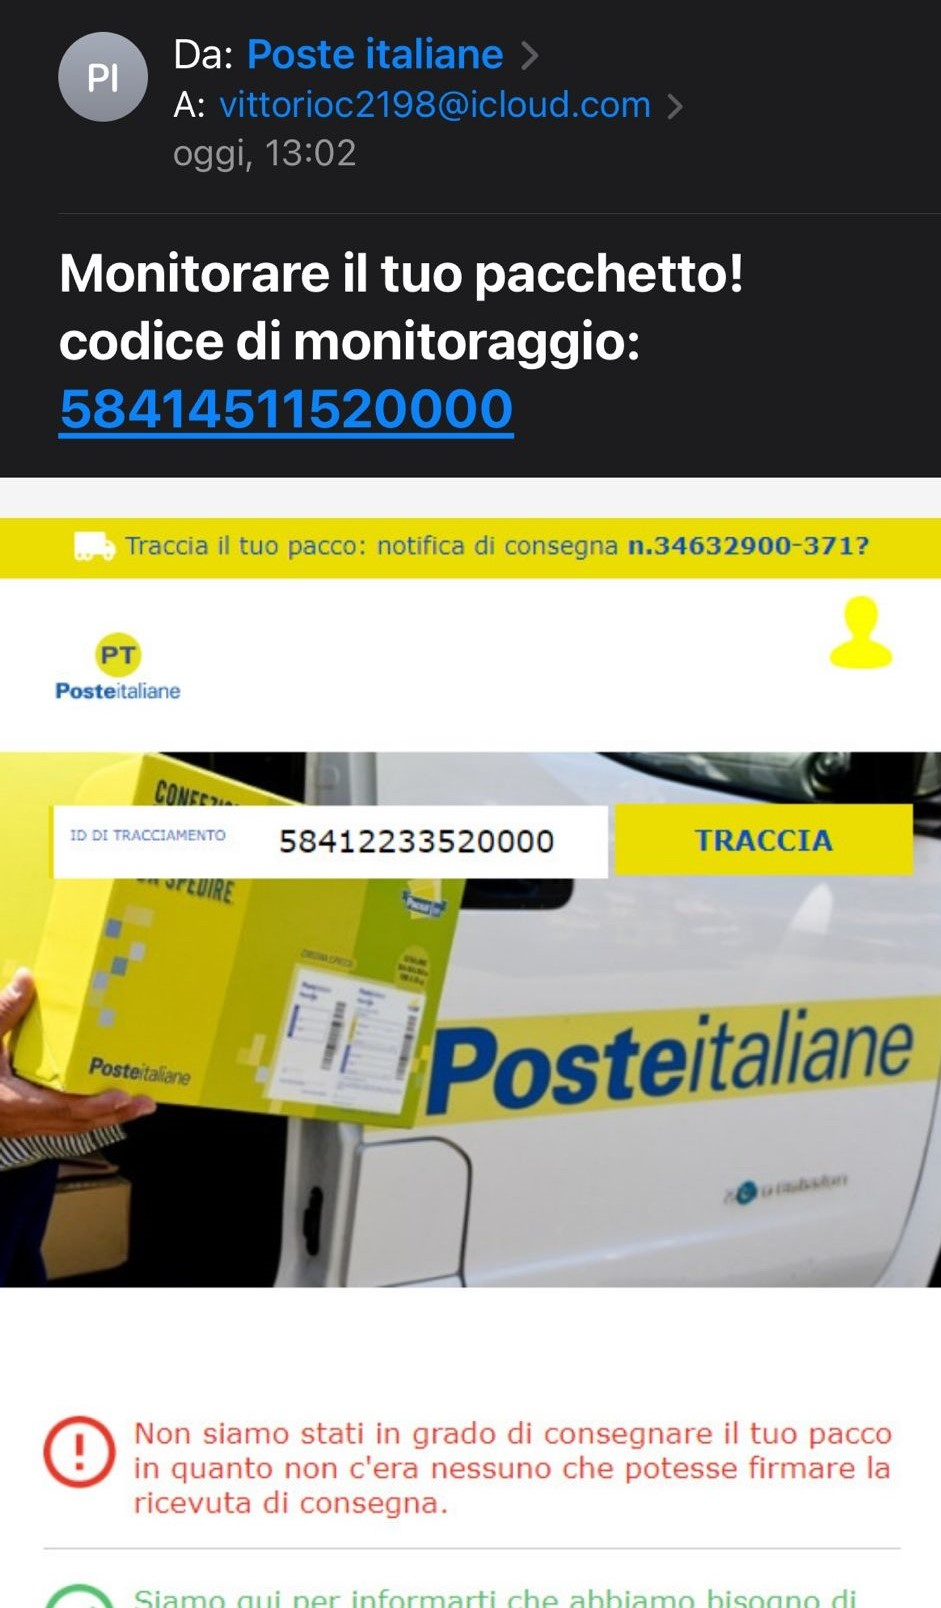
\includegraphics[width=\textwidth]{pictures/phishing1.jpeg}
    \caption{Mail Phisging}
    \label{fig:phish1}
  \end{minipage}
  \hfill
  \begin{minipage}[b]{0.4\textwidth}
    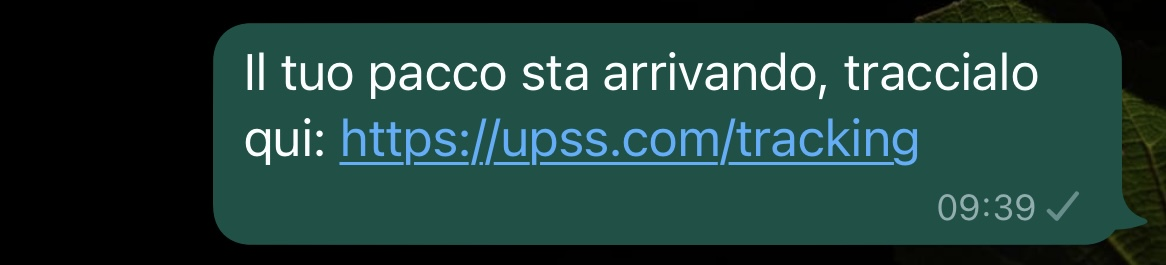
\includegraphics[width=\textwidth]{pictures/phishing2.jpeg}
    \caption{SMS Phishing}
    \label{fig:phish2}
  \end{minipage}
\end{figure}\\
La figura \ref{fig:phish1} mostra un esempio di MAIL phishing mentre la figura \ref{fig:phish2} mostra un esempio di SMS Phishing\\


%% SECTION2
\section{Tipi di squatting}
Per effettuare il phihing, i malintenzionati utilizzano diverse tecniche di cybersquatting. Nella figura \ref{fig:phish2} ad esempio, viene sfruttato quello che viene chiamato "typo-squatting": viene acquistato un dominio che si basa su errori di battitura/digitazione. Come si può notare questo dirotta l'utente verso un sito differente da quello che voleva raggiungere.
Ovviamente le minacce non si circoscrivono solamente a typosquatting.\\
In generale vengono definiti 5 tipi di cybersquatting:
\begin{itemize}
    \item typo: come spiegato sopra, sono quei domini che si basano su errori di battitura e digitazione.
    
    \item homoglyph: questo tipo di squatting invece è uno dei più ingannevoli. Utilizza il fatto che molti caratteri tipografici sono simili tra loro. Nel dominio google, posso sostituire una 'o' con una lettera simile, ad esempio 'ŏ' (goŏgle.com).\\
    Questo tipi di dominio vengono chiamati IDN (internationalized domain name). Sono appunto nomi di dominio che contengono caratteri di alfabeto non latini (cinese, cirillico, greco, etc...). Questi nomi di dominio vengono salvati sui server DNS come stringhe ASCII utilizzando la trascrizione Punycode come visto nella Tabella~\ref{table:tab1}.
    \begin{table}[!h]
        \centering
        \caption{}
        \begin{tabular}{|l|l|}
        \hline
            IDN              & Punycode                     \\ \hline
            www.facebŏŏk.com & www.xn--facebk-tgba.com      \\
            www.googlè.com   & www.xn--googl-8ra.com        \\
        \hline
        \end{tabular}
        \label{table:tab1}
    \end{table}
    
    \item bit: questa forma di cybersquatting si basa su errori di bit-flip che si verificano durante il processo di richiesta DNS. Questi cambi di bit possono verificarsi a causa di fattori quali hardware difettoso o interferenze elettromagntiche.
    
    \item combo: il combosquatting aggiunge termini familiari negli URL che gli utenti incauti potrebbero non notare a prima vista. Questa tecnica si basa su analisi statistiche dei termini più utilizzati nelle pagine di enti affidabili, ad esempio, su instagram si usa molto la parola "story", "stories", "tags". Sapendo questo è possibile creare domini di squatting concatenando il dominio originario con uno dei termini più utilizzati: instagram-stories.com, instagram-tags.com, e così via.
    
    \item wrongTLD: Tutte le tecniche di squatting di cui sopra si
    concentrano sul nome di dominio ma ignorano il TLD. questa tecnica si riferisce a domini che cambiano il TLD ma mantengono il nome di dominio uguale. Per esempio, google.kekw appartiene alla categoria wrongTLD.
\end{itemize}
Sul web\footnote[1]{https://www.catonetworks.com/blog/cato-networks-adds-protection-from-the-perils-of-cybersquatting/} è possibile reperire dati e grafici riguardanti il numero di domini abusati, quale tipologia viene più utilizzata e quale marchio è più preso di mira dai malintenzionati del caso.
La figura \ref{fig:cakesquatting}, ad esempio mostra un grafico a torta che illustra le tipologie più utilizzate.
Ovviamente chi abusa del cybersquatting per commettere crimini come phishing, mira ad utilizzare domini squatted di marchi che statisticamente gli utenti utilizzano più frequentemente o i più indispensabili (come le banche ad esempio). In figura \ref{fig:squatdata} una vista dei marchi che vengono presi più di mira negli ultimi anni.

\begin{figure}[!h]
  \centering
  \begin{minipage}[b]{0.9\textwidth}
    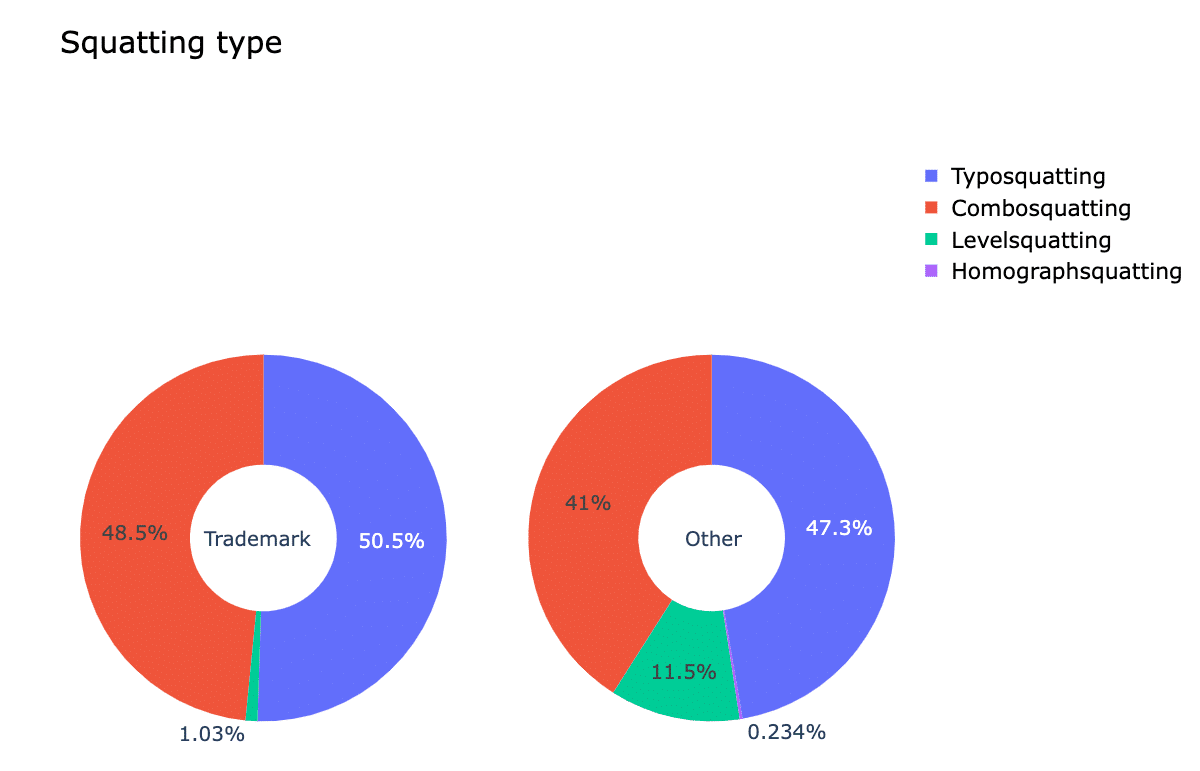
\includegraphics[width=\textwidth]{pictures/cakesquatting.png}
    \caption{Due esempi delle percentuali di squatting più utilizzate. Il primo luogo le percentuali riguardanti i marchi più famosi, in secondo luogo tutti gli altri domini}
    \label{fig:cakesquatting}
  \end{minipage}
  \hfill
\end{figure}

\begin{figure}[!h]
  \centering
  \begin{minipage}[b]{\textwidth}
    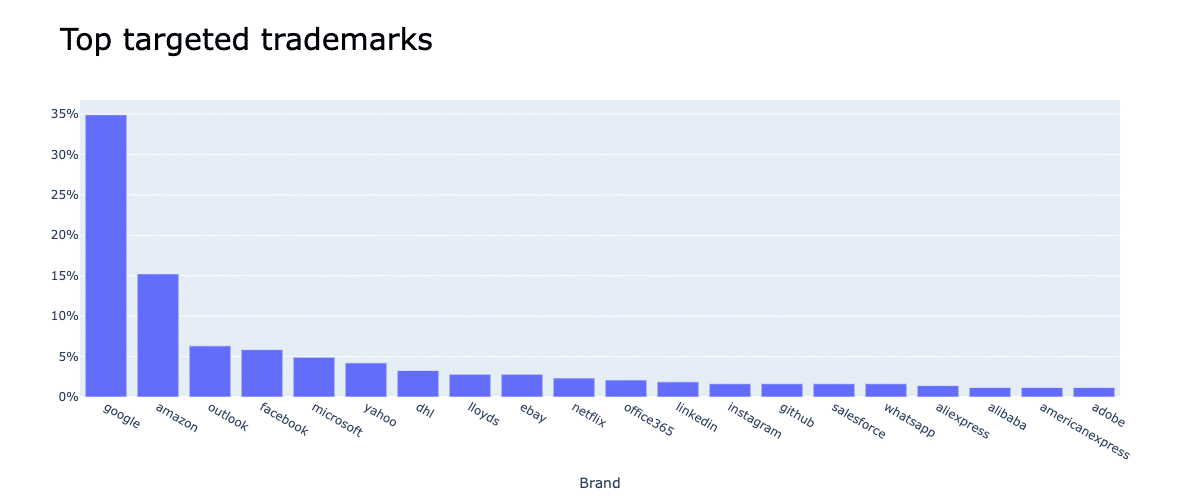
\includegraphics[width=\textwidth]{pictures/squatdata.png}
    \caption{Dati riguardanti i marchi registrati più famosi, e quali di questi vengono più presi di mira dal cybersquatting}
    \label{fig:squatdata}
  \end{minipage}
  \hfill
\end{figure}



\section{Come difendersi}
Per quanto riguarda il phishing attraverso Mail, uno dei modi migliori per difendersi è quello di analizzare il sorgente e di conseguenza analizzare i collegamenti ipertestuali per verificarne la validità. Inoltre, molti antivirus moderni, introducono un modulo per la supervisione in tempo reale delle pagine web che visitiamo: i software antivirus inglobano un modulo che confronta i domini che visitiamo con un database di URL che la compagnia ha etichettato come "malevoli"\cite{inproceedings}.\\
Un altro accorgimento che possiamo adottare è quello di analizzare la semantica e la veridicità delle informazioni[\ref{fig:mailphished}] che, ad esempio, nel caso di un SMS o di una MAIL possono essere alterate facilmente: se si riceve una Mail o un SMS in cui viene indicato che un nostro pacco è stato smarrito, ma non abbiamo ordinato nessun prodotto, è facilmente riconducibile ad un caso di phishing, senza neanche ricondurci ad analizzare il sorgente della MAIL o analizzare l'URL in oggetto.\\
Inoltre, un modo per aggirare il problema alla radice, e quindi avere la minor probabilità possibile di ricevere Mail/SMS Phishing, è proprio quello di evitare di diffondere indirizzi di posta (o numeri di telefono) ad enti/pagine web che non riteniamo del tutto affiabili. Questo perchè nel momento in cui ci iscriviamo ad un forum/applicazione/website in generale, stiamo cedendo i nostri dati alla compagnia che ne gestisce il servizio. Questi dati, nel peggiore dei casi, verranno venduti per altri scopi ad altre compagnie o chissà a chi (evitiamo di iscriverci alle newsletter).\\
In ultimo, ma non meno importante, è ciò che viene chiamato Web Crawler: Un Web crawler (spesso abbreviato in crawler) è un bot Internet che naviga sistematicamente nel World Wide Web e che è tipicamente gestito dai motori di ricerca ai fini dell'indicizzazione del Web. Il problema nasce quando non sono i motori di ricerca che utilizzano il crawling, ma enti a scopo maligno. In sostanza analizzano le pagine del WWW (scrapping) ed estrapolano qualsiasi indirizzo Mail/Numeri di telefono inserendoli successivamente in un database che utilizzeranno per i lor scopi non puliti.\\
Un'esempio più che reale è ciò che è successo a me, dopo aver pubblicato il mio indirizzo Mail sul sito di GitHub (figura \ref{fig:git}). Successivamente a quella mia azione, qualche web crawler avrà fatto scrapping della mia pagina trovando la mia Email all'interno nel sorgente dell'ipertesto (si può notare in figura \ref{fig:git2} la mail estraibile dal sorgente)
\begin{figure}
  \centering
  \begin{minipage}[b]{0.4\textwidth}
    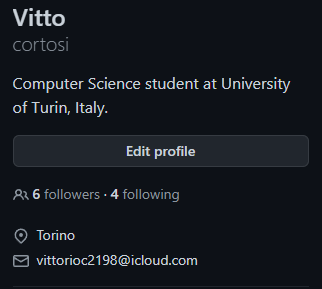
\includegraphics[width=\textwidth]{pictures/git1.png}
    \caption{La Mail inserita da me e resa pubblica sul sito GitHub}
    \label{fig:git}
  \end{minipage}
  \begin{minipage}[b]{0.56\textwidth}
    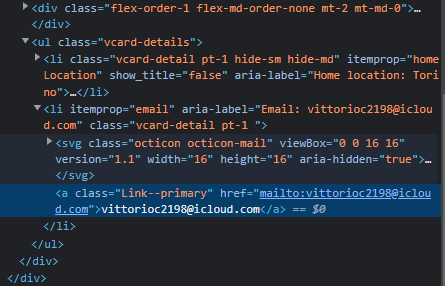
\includegraphics[width=\textwidth]{pictures/git2.png}
    \caption{La Mail che compare nel sorgente della pagina}
    \label{fig:git2}
  \end{minipage}
\end{figure}\\

\begin{figure}[!h]
  \centering
  \begin{minipage}[b]{0.5\textwidth}
    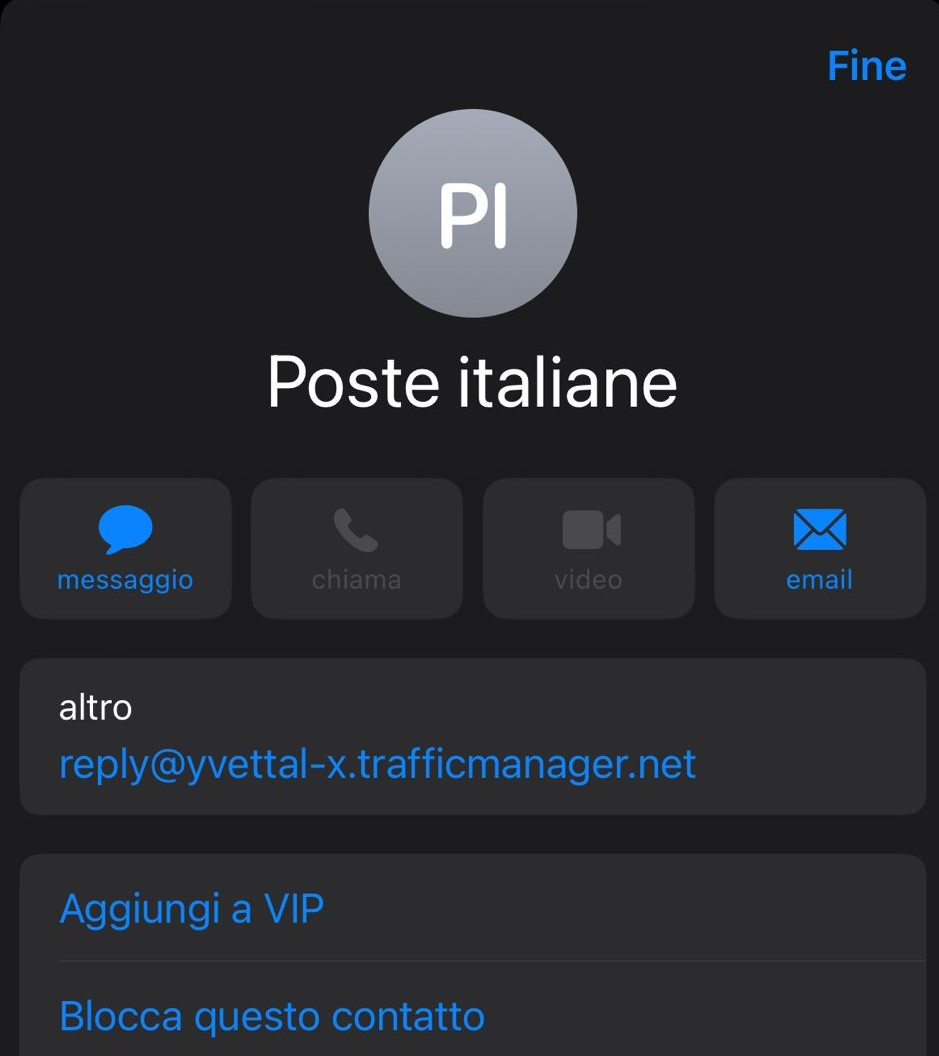
\includegraphics[width=\textwidth]{pictures/phishing3.jpg}
    \caption{In riferimanento alla figura \ref{fig:phish1}, ci si potrebbe difendere andando a controllare l'indirizzo da cui è stata inviata la mail}
    \label{fig:mailphished}
  \end{minipage}
  \hfill
\end{figure}

%% SECTION3
\section{Reti neurali generative}
Costruire un sistema in grado di generare in modo proattivo una quantità considerevole di domini di squatting non è banale. Esistono già sistemi in grado di farlo (DNSTwist è un esempio), ma come indicato dagli autori dall'articolo Needle in a Haystack\cite{10.1145/3278532.3278569}, questi generatori di domini di squatting sono in parte affidabili in quanto sono limitati in quanto non riescono a gestire in modo efficace domini di squatting combinati (combo) o domini che cambiano il TLD, inoltre, gli strumenti esistenti sono molto incompleti nel rilevamento dei domini omografici. Troviamo che strumenti come DNSTwist non riescono a mappare l'elenco completo di caratteri Unicode simili. Ad esempio, ci sono 23 diversi caratteri Unicode che sembrano simili alla lettera "un", ma DNSTwist ne cattura solo 13. Queste limitazioni danneggeranno seriamente le nostre possibilità di catturare pagine di phishing occupate.\\
Uno dei modi per cui si può pensare di generare in modo proattivo dei domini di squatting, è con l'utilizzo di Reti neurali, in particolare, utilizzando reti neurali generative.\\
Le reti neurali generative sono una classe di metodi per l'apprendimento automatico in cui due reti neurali si sfidano diventando uno l'avversario dell'altro (infatti vengono anche chiamate reti neurali generative avversarie). In questo processo, una rete neurale chiamata Generatore genera dati candidati che poi la controparte, chiamata Discriminatore, le valuta. Il generatore quindi cerca di ingannare il discriminatore generando il più possibile dati che rispecchiano quelli reali. Nella figura \ref{fig:gan1} uno schema semplice di GAN\\
\begin{figure}[!h]
  \centering
  \begin{minipage}[b]{\textwidth}
    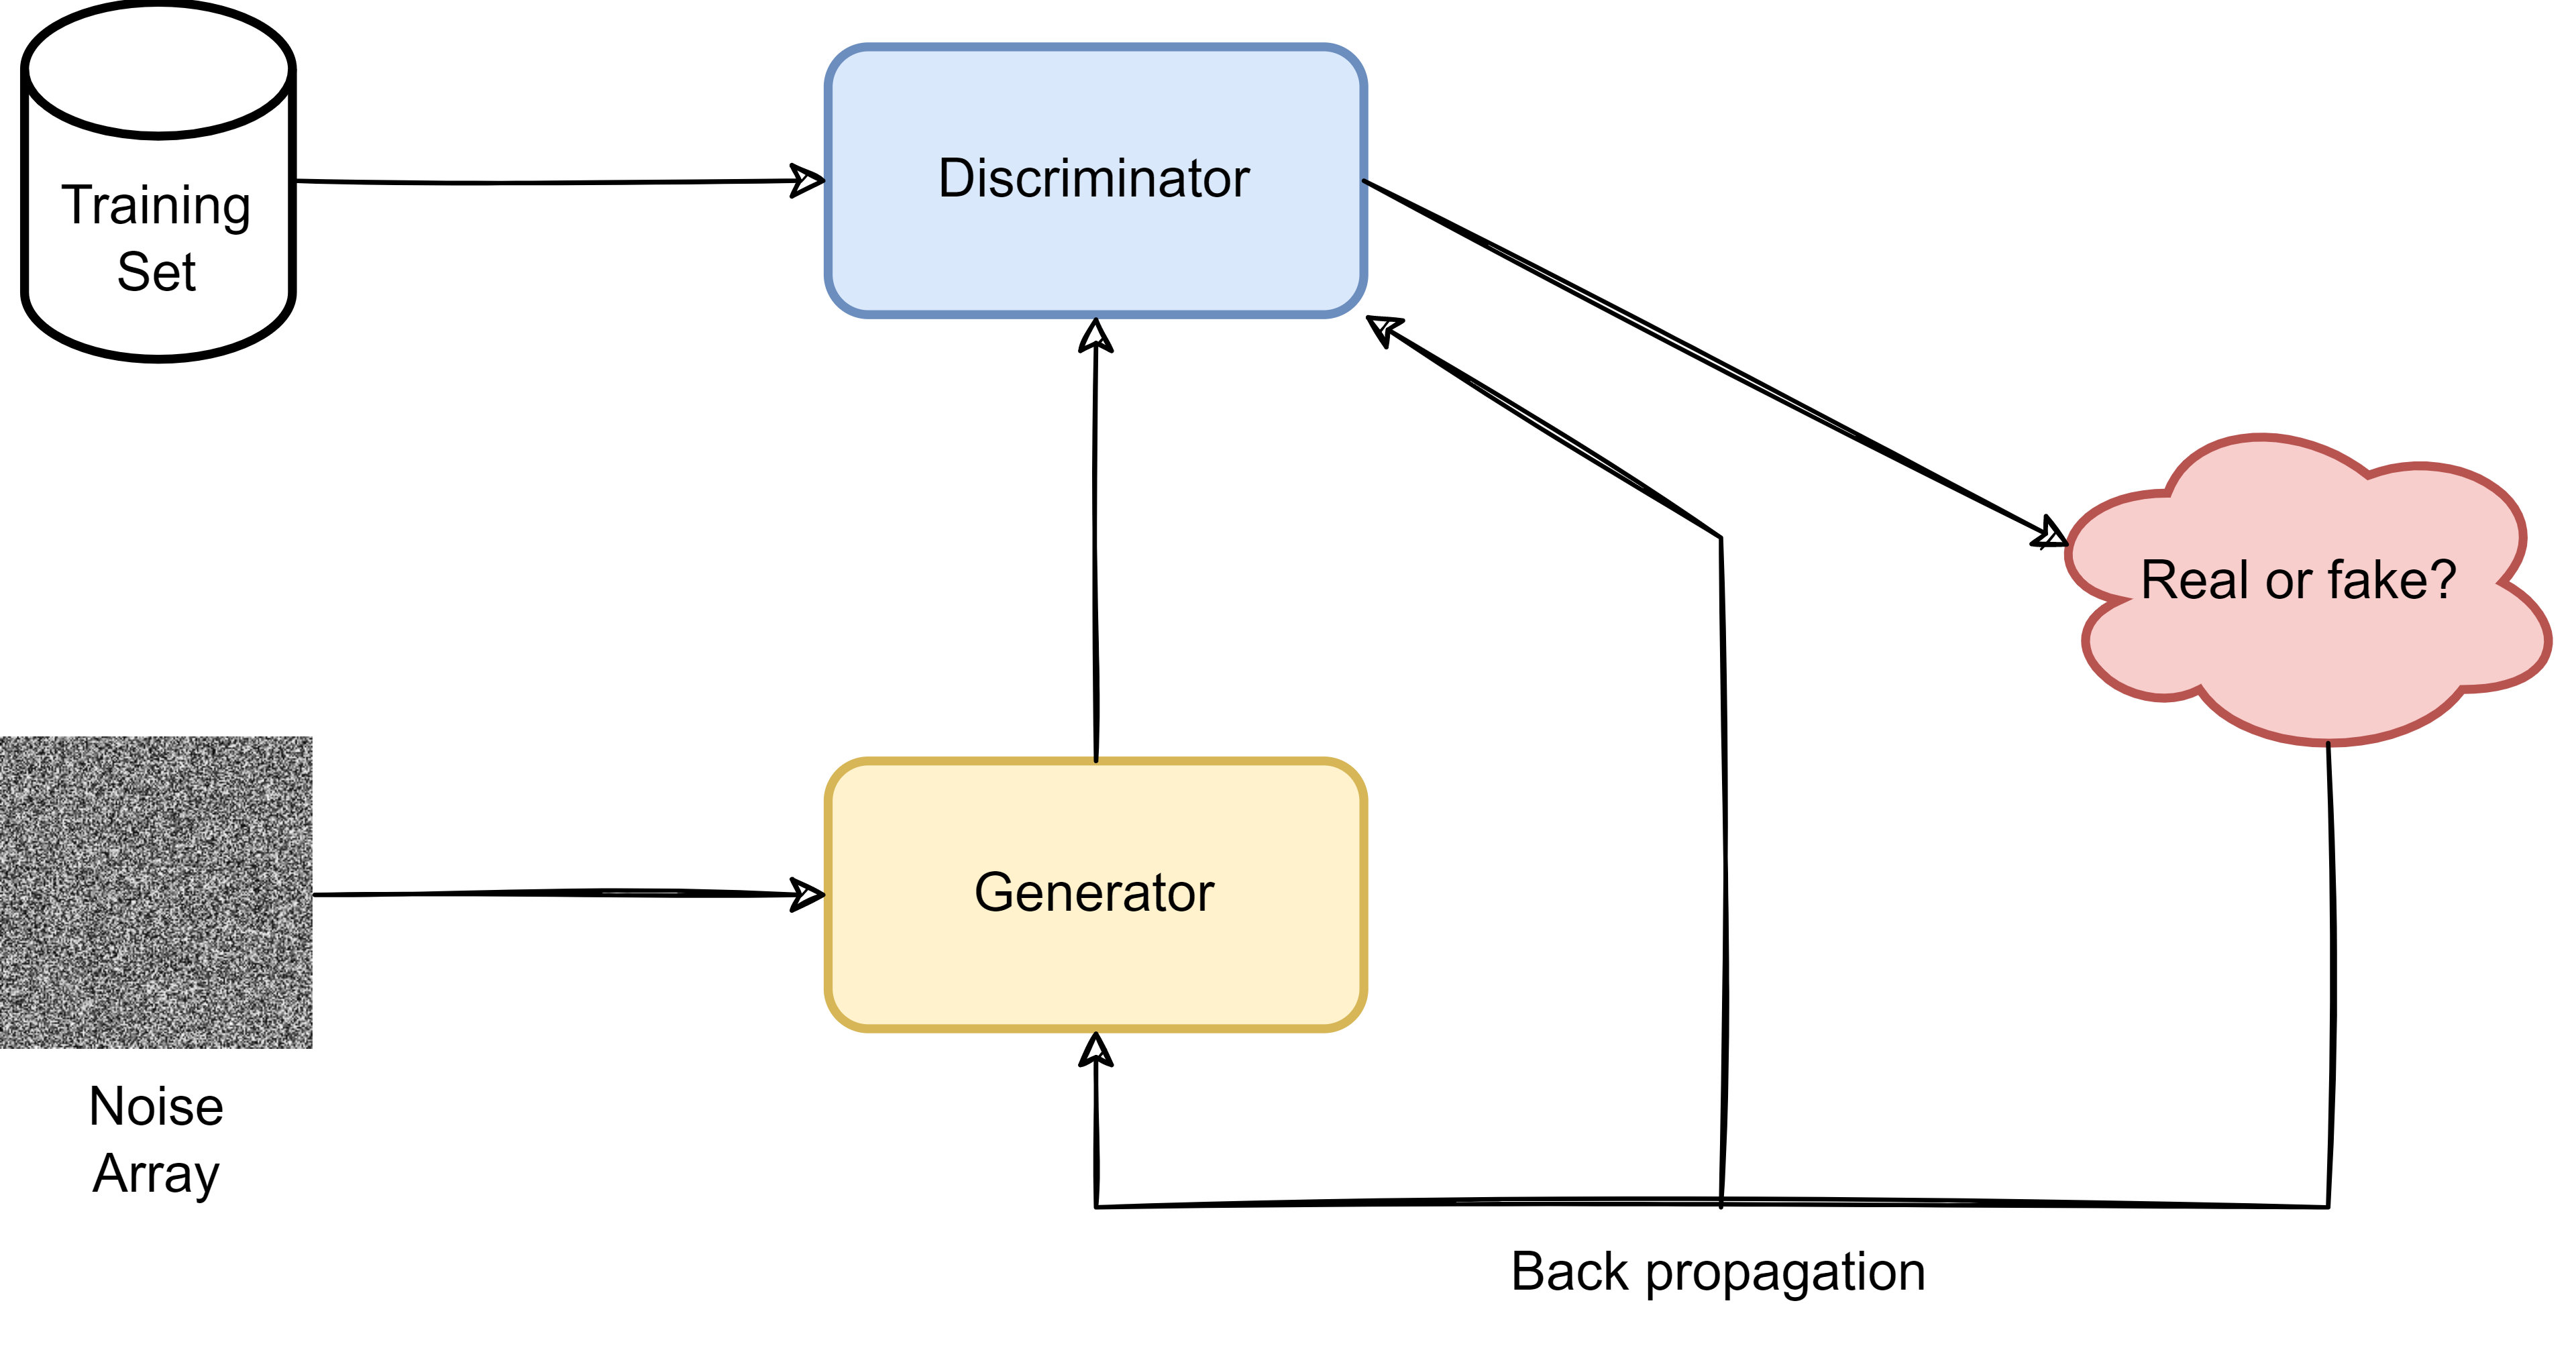
\includegraphics[width=\textwidth]{pictures/gan.png}
    \caption{Simple Gan Scheme}
    \label{fig:gan1}
  \end{minipage}
  \hfill
\end{figure}
Il modello di rete neurale generativa che utilizzerò per la generazione proattiva di domini di squatting, è chiamata Deep Convolutional Generative Adversarial Network

\section{Le DCGAN}
Le reti convoluzionali generative, seguono la filosofia delle reti generative classiche ma procedono utilizzando una struttura dei layer totalmente differente. Nelle reti generative convoluzionali, sia il generatore che il discriminatore utilizzano reti profonde costituite interamente da strati di convoluzione-deconvoluzione, ovvero da qui il nome "rete convoluzionale generativa".\\
Le reti convoluzionali (non per forza generative, CNN) sono utilizzate nell'apprendimento automatico in maniera importante soprattutto per il riconoscimento di immagini.

%% SECTION4
\section{Le GANs nella cybersecurity}
Le applicazioni\cite{9298135} per questi modelli di rete neurale sono davvero molteplici ed il potenziale è davvero enorme, in quanto, questi modelli di reti neurali possono essere istruiti a creare informazioni estremamente simili a qualsiasi dominio della vita reale: immagini, musica, audio, testo.\\
Vengono, inoltre, utilizzati anche nella branca della sicurezza informatica, la cosa meno entusiasmante è che vengono usate in primo luogo come metodo di attacco.\\
In primo luogo vengono utilizzate per eludere sistemi di riconoscimento di Malware: un sistema che genera malware appoggiandosi ad un modello di rete GAN è in grado di generare dei malware che sono non identificabili (o difficilmente) dal sistema su cui dovrà essere eseguito.\\
In secondo luogo possono essere usate per violare sistemi di autenticazione biometrica: sistemi che potrebbero basare i loro permessi di accesso attraverso l'uso della voce o del volto.
Come ultimo esempio, ma non meno importante, è l'applicazione delle GAN nei sistemi di password guessing: l'autenticazione della password è uno dei metodi più comunemente utilizzati dagli utenti che tendono a scegliere password facili da indovinare poichè utilizzano stringhe comuni. Questi tipi di stringhe sono soggetti ad attacchi chiamati password guessing in cui un utente malintenzionato tenta di accedere utilizzando un database di stringhe comuni, dizionari di parole e database di password leaked. L'efficacia dell'attacco si basa sulla capacità di testare rapidamente un gran numero di password altamente probabili rispetto a ciascun hash di password. Una tecnica avanzata si basa sull'intuizione su come gli utenti scelgono le password definendo un'euristica per le trasformazioni delle password, che include combinazioni di più parole e lettere maiuscole e minuscole, etc... Poichè lo sviluppo e il test di nuove regole ed euristiche è un'attività dispendiosa in termini di tempo e che richiede competenze specializzate, entrano in gioco le GANs. Poiché la password è una stringa codificata in testo, è possibile utilizzare un approccio basato su GAN in cui una rete neurale viene addestrata per determinare autonomamente le caratteristiche e le strutture delle password e per sfruttare questa conoscenza per generare nuovi campioni che seguono la stessa distribuzione. Le reti neurali profonde sono sufficientemente espressive da acquisire una gamma di proprietà e strutture che descrivono la maggior parte delle password scelte dall'utente e possono essere addestrate senza alcuna conoscenza o ipotesi pregressa. Ciò implica un'ampia gamma di conoscenze per indovinare le password che includono e superano ciò che viene catturato nelle regole generate dall'uomo e nei processi di generazione delle password.